% 
\documentclass[aspectratio=169]{beamer}
\usetheme{WG}
\usepackage[english,russian]{babel}
\usepackage[utf8]{inputenc}
\usepackage{verbatim}
\usepackage{graphicx}
\usepackage{pgfpages}
\usepackage{ulem}
\usepackage{float}
\usepackage{amsmath}

% quote author
\usepackage{amsthm} % pushQED, popQED
\newenvironment{aquote}[1]{%
  \pushQED{#1}%
  \begin{quote}
}{%
  \noindent\hfill(\popQED)%
  \end{quote}%
}

\definecolor{mygreen}{RGB}{0,150,0}
\definecolor{myyellow}{RGB}{120,120,0}

\usepackage{listings}
\definecolor{light-gray}{gray}{0.95}
\lstset{
language=Python,                             % Code langugage
basicstyle=\small\ttfamily,                   % Code font, Examples: \footnotesize, \ttfamily
keywordstyle=\color{WGred},        % Keywords font ('*' = uppercase)
commentstyle=\color{gray},              % Comments font
numbers=left,                           % Line nums position
numberstyle=\tiny,                      % Line-numbers fonts
stepnumber=1,                           % Step between two line-numbers
numbersep=5pt,                          % How far are line-numbers from code
backgroundcolor=\color{light-gray}, % Choose background color
frame=lines,                             % A frame around the code
tabsize=4,                              % Default tab size
captionpos=b,                           % Caption-position = bottom
breaklines=true,                        % Automatic line breaking?
breakatwhitespace=false,                % Automatic breaks only at whitespace?
showspaces=false,                       % Dont make spaces visible
showstringspaces=false,
stringstyle=\color{myyellow},
showtabs=false,                         % Dont make tabls visible
}

\lstset{emph={yield},emphstyle={\color{WGred}}}
\lstset{emph={self},emphstyle={\color{mygreen}}}


\begin{document}

\title{Про асинхронное сетевое программирование и Python}
\author{Стас Рудаков}
\date{}

{
\title{про асинхронное сетевое программирование}
\titleframe
}


%%%%%%%%%%%%%%%%%%%%%%%%%%%%%%%%%%%%%%%%
%%%%%%%%%%%%%%%%%%%%%%%%%%%%%%%%%%%%%%%%
%%%%%%%%%%%%%%%%%%%%%%%%%%%%%%%%%%%%%%%%
%%%%%%%%%%%%%%%%%%%%%%%%%%%%%%%%%%%%%%%%
%%%%%%%%%%%%%%%%%%%%%%%%%%%%%%%%%%%%%%%%
\begin{frame}
  \frametitle{Да что мы всё обо мне, да обо мне\ldots}
\end{frame}


%%%%%%%%%%%%%%%%%%%%%%%%%%%%%%%%%%%%%%%%
%%%%%%%%%%%%%%%%%%%%%%%%%%%%%%%%%%%%%%%%
%%%%%%%%%%%%%%%%%%%%%%%%%%%%%%%%%%%%%%%%
%%%%%%%%%%%%%%%%%%%%%%%%%%%%%%%%%%%%%%%%
%%%%%%%%%%%%%%%%%%%%%%%%%%%%%%%%%%%%%%%%
\begin{frame}
  \frametitle{О чем будем говорить}
  \begin{columns}
    \begin{column}{.5\textwidth}
      \begin{itemize}
        \item Что нам дает асинхронность
        \item Как это работает
        \item Twisted
        \item Gevent
        \item Tornado
        \item PEP 3156
      \end{itemize}
    \end{column}

    \hfill

    \begin{column}{.3\textwidth}
      
\includegraphics[scale=0.08]{img/qrcode.png}
    \end{column}
  \end{columns}

  \vspace{1cm}
  \begin{center}
    \url{https://raw.github.com/nott/talks/master/async.pdf}
  \end{center}
\end{frame}


%%%%%%%%%%%%%%%%%%%%%%%%%%%%%%%%%%%%%%%%
%%%%%%%%%%%%%%%%%%%%%%%%%%%%%%%%%%%%%%%%
%%%%%%%%%%%%%%%%%%%%%%%%%%%%%%%%%%%%%%%%
%%%%%%%%%%%%%%%%%%%%%%%%%%%%%%%%%%%%%%%%
%%%%%%%%%%%%%%%%%%%%%%%%%%%%%%%%%%%%%%%%
\begin{frame}[fragile]
  \frametitle{Работа с сетью: зачем что-то изобретать?}

  \begin{columns}
    \begin{column}{.8\textwidth}
      
      \begin{lstlisting}[caption=urllib\_example.py]
#!/usr/bin/env python2
import urllib2
f = urllib2.urlopen('http://python.org/')
print f.read(10)
      \end{lstlisting}

      \pause

      \begin{lstlisting}[language=sh]
$ time python urllib_example.py 
<!DOCTYPE 

real	0m0.384s
user	0m0.067s
sys	0m0.017s
      \end{lstlisting}

    \end{column}
    \hfill
    \pause

    \begin{column}{.18\textwidth}
      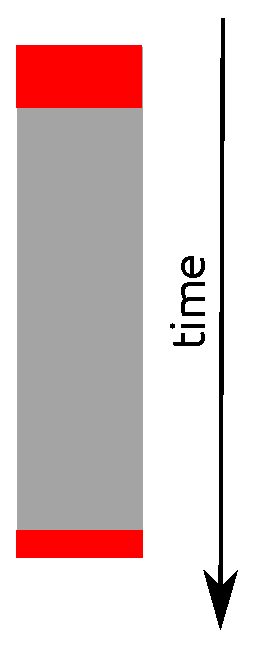
\includegraphics[scale=0.6]{img/part1_1_single.eps}
    \end{column}
  \end{columns}
\end{frame}


%%%%%%%%%%%%%%%%%%%%%%%%%%%%%%%%%%%%%%%%
%%%%%%%%%%%%%%%%%%%%%%%%%%%%%%%%%%%%%%%%
%%%%%%%%%%%%%%%%%%%%%%%%%%%%%%%%%%%%%%%%
%%%%%%%%%%%%%%%%%%%%%%%%%%%%%%%%%%%%%%%%
%%%%%%%%%%%%%%%%%%%%%%%%%%%%%%%%%%%%%%%%
\begin{frame}[fragile]
  \frametitle{Работа с сетью: дальше будет только хуже}

  \begin{columns}
    \begin{column}{.8\textwidth}

      \begin{lstlisting}[caption=urllib\_example2.py]
#!/usr/bin/env python2
import sys
import urllib2
for i in xrange(5):
    f = urllib2.urlopen('http://python.org/')
    print f.read(10),
      \end{lstlisting}

      \pause

      \begin{lstlisting}[language=sh]
$ time python urllib_example2.py
<!DOCTYPE  <!DOCTYPE  <!DOCTYPE

real	0m1.007s
user	0m0.050s
sys	0m0.003s
      \end{lstlisting}
    
    \end{column}
    \hfill
    \pause

    \begin{column}{.18\textwidth}
      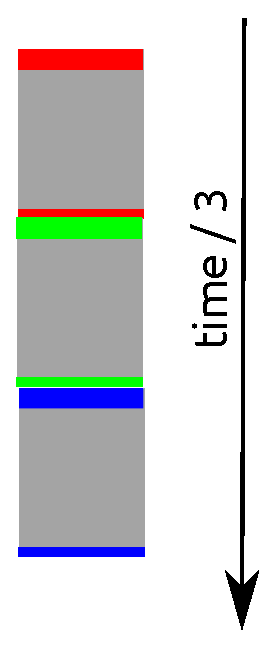
\includegraphics[scale=0.6]{img/part1_2_sequence.eps}
    \end{column}
  \end{columns}
\end{frame}


%%%%%%%%%%%%%%%%%%%%%%%%%%%%%%%%%%%%%%%%
%%%%%%%%%%%%%%%%%%%%%%%%%%%%%%%%%%%%%%%%
%%%%%%%%%%%%%%%%%%%%%%%%%%%%%%%%%%%%%%%%
%%%%%%%%%%%%%%%%%%%%%%%%%%%%%%%%%%%%%%%%
%%%%%%%%%%%%%%%%%%%%%%%%%%%%%%%%%%%%%%%%
\begin{frame}
  \frametitle{I know, I'll use\ldots}

  \begin{columns}
    \begin{column}{.8\textwidth}

      \begin{center}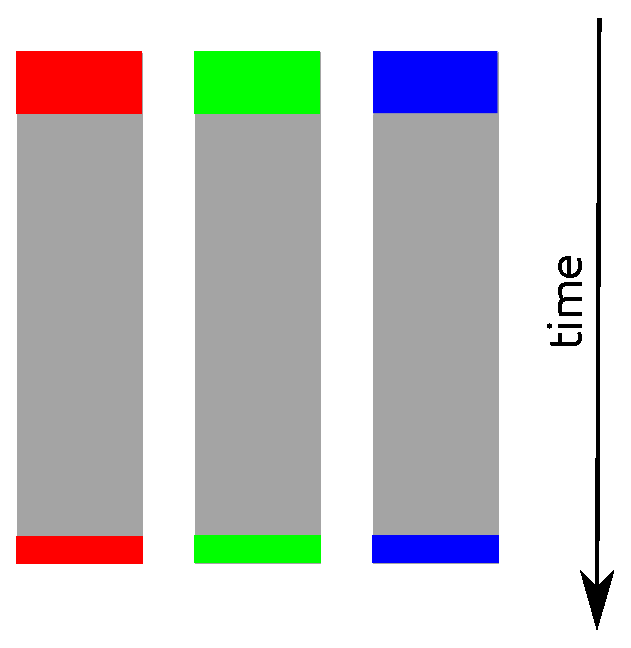
\includegraphics[scale=0.45]{img/part1_3_threads.eps}\end{center}
      \pause

      \begin{aquote}{Ned Batchelder}
        Some people, when confronted with a problem, think,\\
        "I know, I'll use threads,"\\
        and then two they hav erpoblesms.
      \end{aquote}

    \end{column}
    \hfill
    \pause

    \begin{column}{.2\textwidth}
      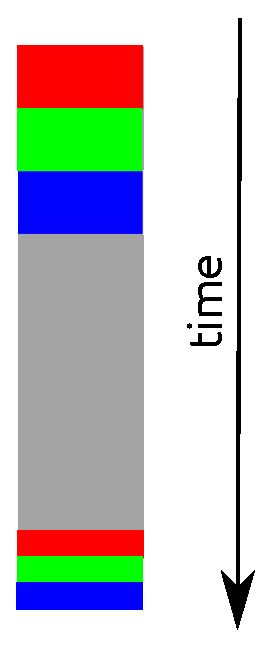
\includegraphics[scale=0.45]{img/part1_4_concurrent.eps}
      \vspace{1.7cm}
    \end{column}
  \end{columns}
\end{frame}


%%%%%%%%%%%%%%%%%%%%%%%%%%%%%%%%%%%%%%%%
%%%%%%%%%%%%%%%%%%%%%%%%%%%%%%%%%%%%%%%%
%%%%%%%%%%%%%%%%%%%%%%%%%%%%%%%%%%%%%%%%
%%%%%%%%%%%%%%%%%%%%%%%%%%%%%%%%%%%%%%%%
%%%%%%%%%%%%%%%%%%%%%%%%%%%%%%%%%%%%%%%%
\begin{frame}
  \frametitle{Apache vs Nginx}
  \pause

  \begin{columns}
    \begin{column}{.45\textwidth}

      \begin{center}Apache\end{center}
      \begin{center}
        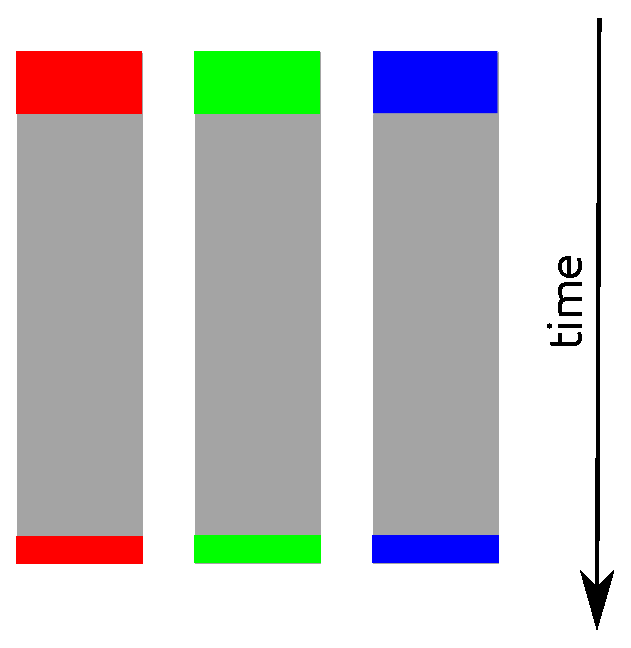
\includegraphics[scale=0.45]{img/part1_3_threads.eps}
      \end{center}

    \end{column}
    \hfill

    \begin{column}{.45\textwidth}
      \begin{center}Nginx\end{center}
      \begin{center}
        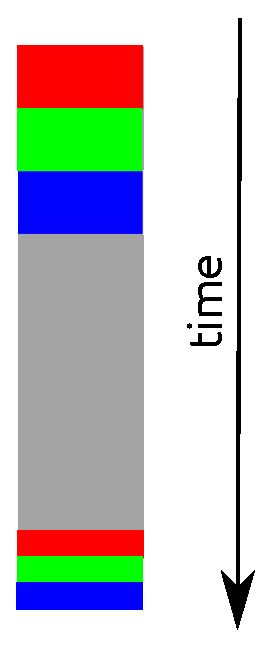
\includegraphics[scale=0.45]{img/part1_4_concurrent.eps}
      \end{center}

    \end{column}
  \end{columns}
\end{frame}


%%%%%%%%%%%%%%%%%%%%%%%%%%%%%%%%%%%%%%%%
%%%%%%%%%%%%%%%%%%%%%%%%%%%%%%%%%%%%%%%%
%%%%%%%%%%%%%%%%%%%%%%%%%%%%%%%%%%%%%%%%
%%%%%%%%%%%%%%%%%%%%%%%%%%%%%%%%%%%%%%%%
%%%%%%%%%%%%%%%%%%%%%%%%%%%%%%%%%%%%%%%%
\begin{frame}[t]
  \frametitle{Лампочка}
  \begin{center}
    
\includegraphics[scale=0.3]{img/part2_1_bulb.eps}
  \end{center}
\end{frame}


%%%%%%%%%%%%%%%%%%%%%%%%%%%%%%%%%%%%%%%%
%%%%%%%%%%%%%%%%%%%%%%%%%%%%%%%%%%%%%%%%
%%%%%%%%%%%%%%%%%%%%%%%%%%%%%%%%%%%%%%%%
%%%%%%%%%%%%%%%%%%%%%%%%%%%%%%%%%%%%%%%%
%%%%%%%%%%%%%%%%%%%%%%%%%%%%%%%%%%%%%%%%
\begin{frame}[t]
  \frametitle{Event loop}
  \begin{center}
    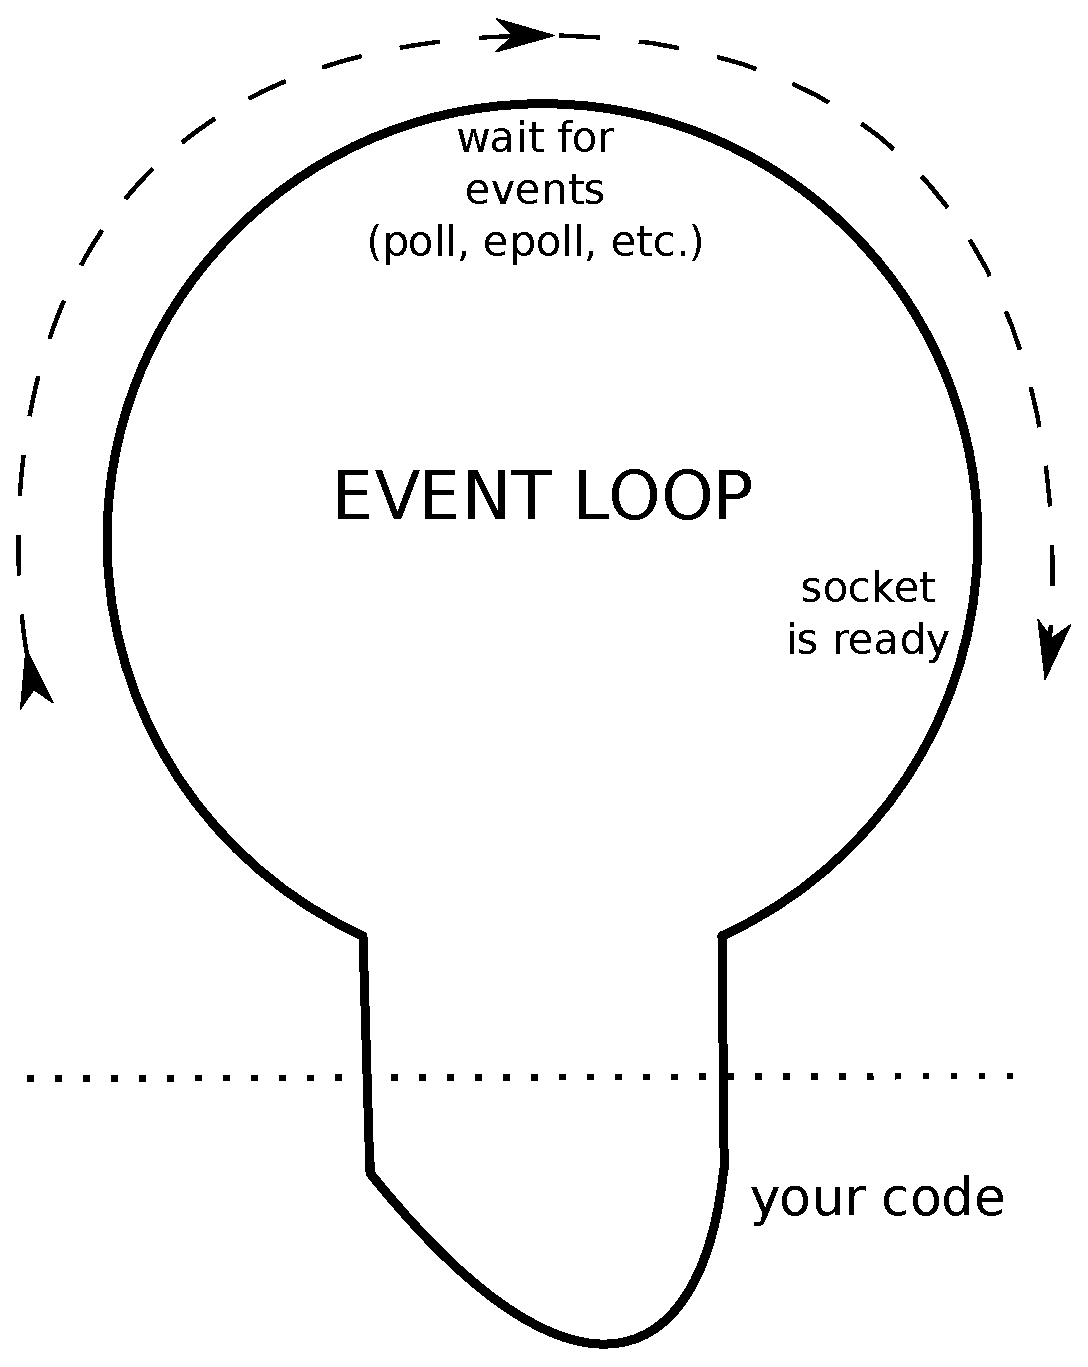
\includegraphics[scale=0.3]{img/part2_2_eventloop.eps}
  \end{center}
\end{frame}


%%%%%%%%%%%%%%%%%%%%%%%%%%%%%%%%%%%%%%%%
%%%%%%%%%%%%%%%%%%%%%%%%%%%%%%%%%%%%%%%%
%%%%%%%%%%%%%%%%%%%%%%%%%%%%%%%%%%%%%%%%
%%%%%%%%%%%%%%%%%%%%%%%%%%%%%%%%%%%%%%%%
%%%%%%%%%%%%%%%%%%%%%%%%%%%%%%%%%%%%%%%%
\begin{frame}[fragile]
  \frametitle{Event loop in GUI}
  \begin{lstlisting}
    def OnClose(self, event):
        dlg = wx.MessageDialog(self,
            "Do you really want to close this application?",
            "Confirm Exit", wx.OK|wx.CANCEL|wx.ICON_QUESTION)
        result = dlg.ShowModal()
        dlg.Destroy()
        if result == wx.ID_OK:
            self.Destroy()
  \end{lstlisting}
  \begin{center}
    
\includegraphics[scale=0.5]{img/part3_dialog.png}
  \end{center}
\end{frame}


%%%%%%%%%%%%%%%%%%%%%%%%%%%%%%%%%%%%%%%%
%%%%%%%%%%%%%%%%%%%%%%%%%%%%%%%%%%%%%%%%
%%%%%%%%%%%%%%%%%%%%%%%%%%%%%%%%%%%%%%%%
%%%%%%%%%%%%%%%%%%%%%%%%%%%%%%%%%%%%%%%%
%%%%%%%%%%%%%%%%%%%%%%%%%%%%%%%%%%%%%%%%
\begin{frame}
  \begin{center}
\includegraphics[scale=0.15]{img/TwistedLogo.eps}\end{center}
  \begin{center}{\Huge Twisted}\end{center}
\end{frame}


%%%%%%%%%%%%%%%%%%%%%%%%%%%%%%%%%%%%%%%%
%%%%%%%%%%%%%%%%%%%%%%%%%%%%%%%%%%%%%%%%
%%%%%%%%%%%%%%%%%%%%%%%%%%%%%%%%%%%%%%%%
%%%%%%%%%%%%%%%%%%%%%%%%%%%%%%%%%%%%%%%%
%%%%%%%%%%%%%%%%%%%%%%%%%%%%%%%%%%%%%%%%
\begin{frame}
  \frametitle{Twisted: transport vs protocol}
  \begin{columns}
    \begin{column}{.45\textwidth}
      Транспорт
      \begin{itemize}
        \item знает, \emph{как} пересылать байты\par
        \item примеры: socket, UNIX pipe, \mbox{SSL socket}, etc.
      \end{itemize}
    \end{column}
    \begin{column}{.45\textwidth}
      Протокол
      \begin{itemize}
        \item знает, \emph{какие} байты пересылать 
        \item примеры: HTTP, SMTP, XMPP, Memcached, etc.
      \end{itemize}
    \end{column}
  \end{columns}
\end{frame}

%%%%%%%%%%%%%%%%%%%%%%%%%%%%%%%%%%%%%%%%
%%%%%%%%%%%%%%%%%%%%%%%%%%%%%%%%%%%%%%%%
%%%%%%%%%%%%%%%%%%%%%%%%%%%%%%%%%%%%%%%%
%%%%%%%%%%%%%%%%%%%%%%%%%%%%%%%%%%%%%%%%
%%%%%%%%%%%%%%%%%%%%%%%%%%%%%%%%%%%%%%%%
\begin{frame}[fragile]
  \frametitle{Twisted: transport vs protocol на примере}
  \begin{lstlisting}
#!/usr/bin/env python2
from twisted.internet import reactor, protocol
class Counter(protocol.Protocol):
    def __init__(self, factory):
        self.factory = factory
    def connectionMade(self):
        num = self.factory.num = self.factory.num + 1 
        self.transport.write("open connections: %d\n" % num)
    def connectionLost(self, reason):
        self.factory.num -= 1
    dataReceived = lambda self, data: None
class CounterFactory(protocol.Factory):
    def __init__(self):
        self.num = 0
    buildProtocol = lambda self, addr: Counter(self)
reactor.listenTCP(8123, CounterFactory())
reactor.run()
  \end{lstlisting}
\end{frame}


%%%%%%%%%%%%%%%%%%%%%%%%%%%%%%%%%%%%%%%%
%%%%%%%%%%%%%%%%%%%%%%%%%%%%%%%%%%%%%%%%
%%%%%%%%%%%%%%%%%%%%%%%%%%%%%%%%%%%%%%%%
%%%%%%%%%%%%%%%%%%%%%%%%%%%%%%%%%%%%%%%%
%%%%%%%%%%%%%%%%%%%%%%%%%%%%%%%%%%%%%%%%
\begin{frame}[fragile]
  \frametitle{Twisted: transport vs protocol}
  \begin{lstlisting}[language=sh]
$ telnet 127.0.0.1 8123
Trying 127.0.0.1...
Connected to 127.0.0.1.
Escape character is '^]'.
open connections: 2
  \end{lstlisting}
\end{frame}


%%%%%%%%%%%%%%%%%%%%%%%%%%%%%%%%%%%%%%%%
%%%%%%%%%%%%%%%%%%%%%%%%%%%%%%%%%%%%%%%%
%%%%%%%%%%%%%%%%%%%%%%%%%%%%%%%%%%%%%%%%
%%%%%%%%%%%%%%%%%%%%%%%%%%%%%%%%%%%%%%%%
%%%%%%%%%%%%%%%%%%%%%%%%%%%%%%%%%%%%%%%%
\begin{frame}
  \frametitle{Twisted: Deferred}
  \begin{itemize}
  \item Deferred --- обещание вернуть результат.
  \item К нему прикрепляются callback'и и errback'и.
  \item Само использование Deferred еще не делает программу асинхронной.
  \item Важно, чтобы callback'и вызывались по событиям (в любых смыслах).
  \end{itemize}
\end{frame}


%%%%%%%%%%%%%%%%%%%%%%%%%%%%%%%%%%%%%%%%
%%%%%%%%%%%%%%%%%%%%%%%%%%%%%%%%%%%%%%%%
%%%%%%%%%%%%%%%%%%%%%%%%%%%%%%%%%%%%%%%%
%%%%%%%%%%%%%%%%%%%%%%%%%%%%%%%%%%%%%%%%
%%%%%%%%%%%%%%%%%%%%%%%%%%%%%%%%%%%%%%%%
\begin{frame}[fragile]
  \frametitle{Twisted: Deferred на примере}
  \begin{lstlisting}[caption=twisted\_example.py]
#!/usr/bin/env python2
import sys
from twisted.internet import defer, reactor
from twisted.python.util import println
from twisted.web.client import getPage

results = []
for i in xrange(int(sys.argv[1])):
    d = getPage('http://www.python.org/')
    d.addCallback(lambda value: value[:10])
    d.addCallback(lambda value: println(value[::-1]))
    d.addErrback(lambda error: println("error:", error))
    results.append(d)

d_list = defer.DeferredList(results)
d_list.addBoth(lambda ignored: reactor.stop())
reactor.run()
  \end{lstlisting}
\end{frame}


%%%%%%%%%%%%%%%%%%%%%%%%%%%%%%%%%%%%%%%%
%%%%%%%%%%%%%%%%%%%%%%%%%%%%%%%%%%%%%%%%
%%%%%%%%%%%%%%%%%%%%%%%%%%%%%%%%%%%%%%%%
%%%%%%%%%%%%%%%%%%%%%%%%%%%%%%%%%%%%%%%%
%%%%%%%%%%%%%%%%%%%%%%%%%%%%%%%%%%%%%%%%
\begin{frame}[fragile]
  \frametitle{Twisted: Deferred}
  \begin{lstlisting}[language=sh]
$ time python twisted_example.py 1
 EPYTCOD!<

real	0m0.833s
user	0m0.250s
sys	0m0.030s
$ time python twisted_example.py 5
 EPYTCOD!<
 EPYTCOD!<
 EPYTCOD!<
 EPYTCOD!<
 EPYTCOD!<

real	0m1.116s
user	0m0.257s
sys	0m0.043s
  \end{lstlisting}
\end{frame}


%%%%%%%%%%%%%%%%%%%%%%%%%%%%%%%%%%%%%%%%
%%%%%%%%%%%%%%%%%%%%%%%%%%%%%%%%%%%%%%%%
%%%%%%%%%%%%%%%%%%%%%%%%%%%%%%%%%%%%%%%%
%%%%%%%%%%%%%%%%%%%%%%%%%%%%%%%%%%%%%%%%
%%%%%%%%%%%%%%%%%%%%%%%%%%%%%%%%%%%%%%%%
\begin{frame}
  \frametitle{Twisted: параллельная вселенная}
  \begin{itemize}
    \item последовательность синхронных операторов $\approx$ цепочка {\tt Deferred};
    \item вызов функции внутри функции $\approx$ возврат {\tt Deferred} из {\tt Deferred};
    \item {\tt Deferred} $\approx$ {\tt stack frame};
    \item блок {\tt try..except} $\approx$ цепочка {\tt errback}'ов;
    \item {\tt threading.join}  $\approx$ {\tt DeferredList};
  \end{itemize}
  \pause

  \vspace{0.5cm}
  \begin{itemize}
    \item {\tt logging};
    \item {\tt plugins};
    \item несовместимость с {\tt stdlib};
    \item отлично проработанная инфраструктура;
    \item достаточно (но далеко не самый) быстрый;
  \end{itemize}

\end{frame}


%%%%%%%%%%%%%%%%%%%%%%%%%%%%%%%%%%%%%%%%
%%%%%%%%%%%%%%%%%%%%%%%%%%%%%%%%%%%%%%%%
%%%%%%%%%%%%%%%%%%%%%%%%%%%%%%%%%%%%%%%%
%%%%%%%%%%%%%%%%%%%%%%%%%%%%%%%%%%%%%%%%
%%%%%%%%%%%%%%%%%%%%%%%%%%%%%%%%%%%%%%%%
\begin{frame}
  \begin{center}
    {\Huge Gevent}

    и прекрасный код
  \end{center}
\end{frame}

%%%%%%%%%%%%%%%%%%%%%%%%%%%%%%%%%%%%%%%%
%%%%%%%%%%%%%%%%%%%%%%%%%%%%%%%%%%%%%%%%
%%%%%%%%%%%%%%%%%%%%%%%%%%%%%%%%%%%%%%%%
%%%%%%%%%%%%%%%%%%%%%%%%%%%%%%%%%%%%%%%%
%%%%%%%%%%%%%%%%%%%%%%%%%%%%%%%%%%%%%%%%
\begin{frame}[fragile]
  \frametitle{Gevent}
  \begin{lstlisting}
#!/usr/bin/python2
import sys
from gevent import joinall, monkey, spawn

monkey.patch_all()

import urllib2

def fetch():
    f = urllib2.urlopen('http://www.python.org/')
    print f.read(10)

num = int(sys.argv[1])
# equivalent can be also implemented with threading
joinall([spawn(fetch) for i in xrange(num)])
  \end{lstlisting}
\end{frame}


%%%%%%%%%%%%%%%%%%%%%%%%%%%%%%%%%%%%%%%%
%%%%%%%%%%%%%%%%%%%%%%%%%%%%%%%%%%%%%%%%
%%%%%%%%%%%%%%%%%%%%%%%%%%%%%%%%%%%%%%%%
%%%%%%%%%%%%%%%%%%%%%%%%%%%%%%%%%%%%%%%%
%%%%%%%%%%%%%%%%%%%%%%%%%%%%%%%%%%%%%%%%
\begin{frame}[fragile]
  \frametitle{Gevent: oh wow!}
  \begin{lstlisting}
$ time python gevent_example.py 1
<!DOCTYPE 

real	0m0.434s
user	0m0.077s
sys	0m0.020s

$ time python gevent_example.py 5
<!DOCTYPE 
<!DOCTYPE 
<!DOCTYPE 
<!DOCTYPE 
<!DOCTYPE 

real	0m0.428s
user	0m0.093s
sys	0m0.023s
  \end{lstlisting}
\end{frame}

%%%%%%%%%%%%%%%%%%%%%%%%%%%%%%%%%%%%%%%%
%%%%%%%%%%%%%%%%%%%%%%%%%%%%%%%%%%%%%%%%
%%%%%%%%%%%%%%%%%%%%%%%%%%%%%%%%%%%%%%%%
%%%%%%%%%%%%%%%%%%%%%%%%%%%%%%%%%%%%%%%%
%%%%%%%%%%%%%%%%%%%%%%%%%%%%%%%%%%%%%%%%
\begin{frame}[fragile]
  \frametitle{Greenlets inside}

  \begin{columns}
    \begin{column}{.48\textwidth}
      \begin{lstlisting}[caption=greenlet\_example.py]
#!/usr/bin/env python
from greenlet import greenlet

def test1():
    print(1)
    gr2.switch()
    print(3)
def test2():
    print(2)
    gr1.switch()
    print(4)

gr1 = greenlet(test1)
gr2 = greenlet(test2)
gr1.switch()
      \end{lstlisting}

    \end{column}%
    \hfill%
    
    \begin{column}{.48\textwidth}
      \begin{lstlisting}[numbers=none]
$ python greenlet_example.py 
1
2
3
      \end{lstlisting}

    \end{column}%
  \end{columns}

\end{frame}


%%%%%%%%%%%%%%%%%%%%%%%%%%%%%%%%%%%%%%%%
%%%%%%%%%%%%%%%%%%%%%%%%%%%%%%%%%%%%%%%%
%%%%%%%%%%%%%%%%%%%%%%%%%%%%%%%%%%%%%%%%
%%%%%%%%%%%%%%%%%%%%%%%%%%%%%%%%%%%%%%%%
%%%%%%%%%%%%%%%%%%%%%%%%%%%%%%%%%%%%%%%%
\begin{frame}
  \frametitle{Gevent: есть нюанс}
  \begin{itemize}
  \item Текущая версия 0.13.
  \item В версии 1.0 запланирован переход с {\tt libevent} на {\tt libev}.
    \pause
  \item Первая $\beta$-версия для 1.0 была выпущена около 2 лет назад.
    \pause
  \item Пугают страшилки про гринлеты.
    \pause
  \item Проблемы с совместимостью с существующими библиотеками.
  \end{itemize}
\end{frame}


%%%%%%%%%%%%%%%%%%%%%%%%%%%%%%%%%%%%%%%%
%%%%%%%%%%%%%%%%%%%%%%%%%%%%%%%%%%%%%%%%
%%%%%%%%%%%%%%%%%%%%%%%%%%%%%%%%%%%%%%%%
%%%%%%%%%%%%%%%%%%%%%%%%%%%%%%%%%%%%%%%%
%%%%%%%%%%%%%%%%%%%%%%%%%%%%%%%%%%%%%%%%
\begin{frame}
  \begin{center}
    {\Huge Tornado}

    и быстрые HTTP серверы
  \end{center}
\end{frame}


%%%%%%%%%%%%%%%%%%%%%%%%%%%%%%%%%%%%%%%%
%%%%%%%%%%%%%%%%%%%%%%%%%%%%%%%%%%%%%%%%
%%%%%%%%%%%%%%%%%%%%%%%%%%%%%%%%%%%%%%%%
%%%%%%%%%%%%%%%%%%%%%%%%%%%%%%%%%%%%%%%%
%%%%%%%%%%%%%%%%%%%%%%%%%%%%%%%%%%%%%%%%
\begin{frame}[fragile]
  \frametitle{Tornado}
  \begin{lstlisting}
#!/usr/bin/env python
import tornado.ioloop
import tornado.httpclient
import tornado.web

class Handler(tornado.web.RequestHandler):
    @tornado.web.asynchronous
    def get(self, path):
        http = tornado.httpclient.AsyncHTTPClient()
        http.fetch("http://www.python.org/" + path,
                   self._on_download)
    def _on_download(self, response):
        self.write(response.body)
        self.finish()
application = tornado.web.Application([(r"/(.*)", Handler),])
application.listen(8888)
tornado.ioloop.IOLoop.instance().start()
  \end{lstlisting}
\end{frame}


%%%%%%%%%%%%%%%%%%%%%%%%%%%%%%%%%%%%%%%%
%%%%%%%%%%%%%%%%%%%%%%%%%%%%%%%%%%%%%%%%
%%%%%%%%%%%%%%%%%%%%%%%%%%%%%%%%%%%%%%%%
%%%%%%%%%%%%%%%%%%%%%%%%%%%%%%%%%%%%%%%%
%%%%%%%%%%%%%%%%%%%%%%%%%%%%%%%%%%%%%%%%
\begin{frame}[fragile]
  \frametitle{Tornado: we need an HTTP client!}
  \begin{lstlisting}
#!/usr/bin/env python
import sys, tornado.ioloop, tornado.httpclient

def fetch():
    http = tornado.httpclient.AsyncHTTPClient()
    http.fetch("http://www.python.org/", on_download)
def on_download(response):
    print(response.body[:10])
    global num
    num -= 1
    if not num: ioloop.stop()

num = int(sys.argv[1])
ioloop = tornado.ioloop.IOLoop.instance()
for i in range(num):
    ioloop.add_callback(fetch)
ioloop.start()
  \end{lstlisting}
\end{frame}


%%%%%%%%%%%%%%%%%%%%%%%%%%%%%%%%%%%%%%%%
%%%%%%%%%%%%%%%%%%%%%%%%%%%%%%%%%%%%%%%%
%%%%%%%%%%%%%%%%%%%%%%%%%%%%%%%%%%%%%%%%
%%%%%%%%%%%%%%%%%%%%%%%%%%%%%%%%%%%%%%%%
%%%%%%%%%%%%%%%%%%%%%%%%%%%%%%%%%%%%%%%%
\begin{frame}[fragile]
  \frametitle{Tornado: the results}
  \begin{lstlisting}
$ time python gevent_example.py 5
<!DOCTYPE 
<!DOCTYPE 
<!DOCTYPE 
<!DOCTYPE 
<!DOCTYPE 

real	0m0.428s
user	0m0.093s
sys	0m0.023s

$ time python tornado_httpclient.py  1
<!DOCTYPE 

real	0m0.469s
user	0m0.163s
sys	0m0.027s
  \end{lstlisting}
\end{frame}


%%%%%%%%%%%%%%%%%%%%%%%%%%%%%%%%%%%%%%%%
%%%%%%%%%%%%%%%%%%%%%%%%%%%%%%%%%%%%%%%%
%%%%%%%%%%%%%%%%%%%%%%%%%%%%%%%%%%%%%%%%
%%%%%%%%%%%%%%%%%%%%%%%%%%%%%%%%%%%%%%%%
%%%%%%%%%%%%%%%%%%%%%%%%%%%%%%%%%%%%%%%%
\begin{frame}
  \begin{center}
    {\Huge PEP 3156}

    Asynchronous IO Support Rebooted
  \end{center}
\end{frame}


%%%%%%%%%%%%%%%%%%%%%%%%%%%%%%%%%%%%%%%%
%%%%%%%%%%%%%%%%%%%%%%%%%%%%%%%%%%%%%%%%
%%%%%%%%%%%%%%%%%%%%%%%%%%%%%%%%%%%%%%%%
%%%%%%%%%%%%%%%%%%%%%%%%%%%%%%%%%%%%%%%%
%%%%%%%%%%%%%%%%%%%%%%%%%%%%%%%%%%%%%%%%
\begin{frame}
  \frametitle{PEP 3156: ключевые моменты}
  \begin{itemize}
    \item Разделение на транспорт и протокол --- как в {\tt Twisted}.
    \item {\tt Future} --- объект обещания --- подсмотрен в {\tt Java Futures}.
    \item API построено на {\tt yield from} (до свидания, Python 2).
    \item {\tt Event loop} --- один на поток.
    \item {\tt Tulip} --- reference implementation.
    \item Вероятно, {\tt Tulip} войдет в Python 3.4 под каким-нибудь скучым именем (осень 2013).
  \end{itemize}
\end{frame}


%%%%%%%%%%%%%%%%%%%%%%%%%%%%%%%%%%%%%%%%
%%%%%%%%%%%%%%%%%%%%%%%%%%%%%%%%%%%%%%%%
%%%%%%%%%%%%%%%%%%%%%%%%%%%%%%%%%%%%%%%%
%%%%%%%%%%%%%%%%%%%%%%%%%%%%%%%%%%%%%%%%
%%%%%%%%%%%%%%%%%%%%%%%%%%%%%%%%%%%%%%%%
\begin{frame}[fragile]
  \frametitle{{\tt yield from} на примере}


  \begin{columns}
    \begin{column}{.48\textwidth}
      \begin{lstlisting}[caption=yield\_from.py]
#!/usr/bin/env python3

def a():
    yield 1
    yield 2
    yield 3
    return 'done_1'

def b():
    done = yield from a()
    print(done)
    return 'done_b'

for i in b():
    print(i)
      \end{lstlisting}

    \end{column}%
    \hfill%
    
    \begin{column}{.48\textwidth}
      \begin{lstlisting}[numbers=none]
$ python yield_from.py 
1
2
3
done_1
      \end{lstlisting}

    \end{column}%
  \end{columns}

\end{frame}


%%%%%%%%%%%%%%%%%%%%%%%%%%%%%%%%%%%%%%%%
%%%%%%%%%%%%%%%%%%%%%%%%%%%%%%%%%%%%%%%%
%%%%%%%%%%%%%%%%%%%%%%%%%%%%%%%%%%%%%%%%
%%%%%%%%%%%%%%%%%%%%%%%%%%%%%%%%%%%%%%%%
%%%%%%%%%%%%%%%%%%%%%%%%%%%%%%%%%%%%%%%%
\begin{frame}[fragile]
  \frametitle{Tulip --- reference implementation}
  \begin{lstlisting}
#!/usr/bin/env python3
import sys
import tulip
import tulip.http

def curl(url):
    response = yield from tulip.http.request('GET', url)
    data = yield from response.read()
    print(data.decode('utf-8', 'replace')[:10])

if __name__ == '__main__':
    loop = tulip.get_event_loop()
    loop.run_until_complete(curl(sys.argv[1]))
  \end{lstlisting}
\end{frame}


%%%%%%%%%%%%%%%%%%%%%%%%%%%%%%%%%%%%%%%%
%%%%%%%%%%%%%%%%%%%%%%%%%%%%%%%%%%%%%%%%
%%%%%%%%%%%%%%%%%%%%%%%%%%%%%%%%%%%%%%%%
%%%%%%%%%%%%%%%%%%%%%%%%%%%%%%%%%%%%%%%%
%%%%%%%%%%%%%%%%%%%%%%%%%%%%%%%%%%%%%%%%
\begin{frame}
  \frametitle{``Эй ты, заканчивай там!''}
  \begin{itemize}
    \item Asynchronous networking --- это правильный инструмент\ldots для правильной задачи.
    \item Python настолько крутой, что допускает как минимум 3 возможных подхода для написания асинхронных сетевых фрэймворков.
    \item PEP 3156 выглядит многообещающе.
      \pause
    \item Стас, ты забыл рассказать про совместимость на уровне event loop'ов!
  \end{itemize}
\end{frame}


%%%%%%%%%%%%%%%%%%%%%%%%%%%%%%%%%%%%%%%%
%%%%%%%%%%%%%%%%%%%%%%%%%%%%%%%%%%%%%%%%
%%%%%%%%%%%%%%%%%%%%%%%%%%%%%%%%%%%%%%%%
%%%%%%%%%%%%%%%%%%%%%%%%%%%%%%%%%%%%%%%%
%%%%%%%%%%%%%%%%%%%%%%%%%%%%%%%%%%%%%%%%
\begin{finalframe}
  \frametitle{СПАСИБО ЗА ВНИМАНИЕ. ВОПРОСЫ?}
    \begin{block}{Стас Рудаков}
    \par \url{mailto:stas@garage22.net}
    \par \url{mailto:s_rudakou@wargaming.net}
    \par \url{https://raw.github.com/nott/talks/master/async.pdf}
    \end{block}

    \begin{block}
    \par \url{http://twistedmatrix.com/}
    \par \url{http://www.tornadoweb.org}
    \par \url{http://www.gevent.org/}
    \par \url{http://www.python.org/dev/peps/pep-3156/}
    \par \url{https://code.google.com/p/tulip/}
    \end{block}

\end{finalframe}

\end{document}

